\documentclass[xcolor={usenames,svgnames,x11names,dvipsnames,table}]{beamer}

\usetheme{SBUclass}

\usepackage{mypackages}
\usepackage{mycommands}

\title{\texorpdfstring{Language \& Technology}{Language and Technology}}
\subtitle{Lecture 8: Machine Learning}
\author{Al{\"e}na Aks{\"e}nova \& Aniello De Santo}
\institute{Stony Brook University\\\texttt{alena.aksenova@stonybrook.edu}\\\texttt{aniello.desanto@stonybrook.edu}}
\date{}

\begin{document}

\unnumbered{

\begin{frame}{Reminder: Plan for Remaining Weeks}
    \centering
    \begin{tabular}{rll}
        \toprule
        \textbf{Date} & \textbf{Topic} & \textbf{Hw?}\\
        \midrule
       April  8  & n-gram models & yes {\color{purple}{\checkmark}}\\
       April  10  & Python (functions) \\
        \midrule
        April  15 &  n-gram models (cont.) & yes {\color{purple}{\checkmark}}\\
       April  17 & Python (tokens) \\
        \midrule
       April 22 & Machine learning &yes {\color{purple}{$\Leftarrow$}}\\
        April  24 & Python (ngrams)\\
        \midrule
       April  29 &  Human-like models  & practice/Final project  \\
       May 01 & Python (frequencies)\\
        \midrule
        May 06 & Summary & Final project  \\
        May 08 & Python Q\&A session\\
            \midrule
        May 14 & & Final Project due (at midnight)\\
        
        \bottomrule
    \end{tabular}
\end{frame}
\begin{frame}
	\titlepage
\end{frame}
}

\begin{frame}{Why Machine Learning?}
    \begin{itemize}
        \item For many tasks, designing models by hand is
            \begin{itemize}
                \item too expensive (thousands of man hours), and\slash or
                \item too inflexible (cannot adapt to changes), and\slash or
                \item simply impossible
            \end{itemize}
    \end{itemize}

    \begin{example}
        \begin{itemize}
            \item spam filter
            \item broad-coverage grammars for hundreds of languages
            \item machine translation systems
        \end{itemize}
    \end{example}

    \begin{itemize}
        \item Computers have to be able to learn from input on their own.
        \item \textbf{Also:} Humans learn, too; we don't get English with our genes.
    \end{itemize}
\end{frame}

\begin{frame}{What is Learning?}
    All of the following are colloquially called ``learning'',\\
    but they are \highlight{not the same}:
    %
    \begin{itemize}
        \item learning to walk
        \item learning the names of all US presidents
        \item learning self-discipline
        \item learning tennis
        \item learning addition
        \item learning French (as a second language)
    \end{itemize}
\end{frame}

\begin{frame}{Parameters for Types of Learning}
    \begin{center}
        \begin{tabular}{rcccc}
                                 & \textbf{instruction} & \textbf{end state} & \textbf{generalization} & \textbf{categorical}\\
            \textbf{walking} & \no & \yes & \no & ?\\
            \textbf{presidents} & \yes & \yes & \no & \yes\\
            \textbf{discipline} & \no & \no & \no & \no\\
            \textbf{Tennis} & \yes & ? & ? & ?\\
            \textbf{addition} & \yes & \yes & \yes & \yes\\
            \textbf{French} & \yes & ? & \yes & \no \\
        \end{tabular}
    \end{center}
\end{frame}

\begin{frame}{Learning as Generalization}
    \begin{description}
        \item[learning] generalization from a finite set of inputs to\\
            a (possibly infinite) target class of outputs
    \end{description}

    \begin{block}<2->{The \emph{Gavagai} Problem}
        \begin{itemize}
            \item Suppose you are on a remote island, trying to learn the language of the locals.
            \item One of them points at a rabbit that just jumped out of the bushes and says ``gavagai''.
        \end{itemize}
        \begin{columns}
            \column{.5\linewidth}
            \begin{itemize}
                \item What does \emph{gavagai} mean?
                    \visible<3->{
                        \begin{itemize}
                            \item rabbit
                            \item animal
                            \item Look there!
                            \item Watch out!
                            \item How cute!
                            \item There's our dinner!
                            \item Pull my finger!
                        \end{itemize}
                    }
            \end{itemize}

            \column{.4\linewidth}
            \includegraphics<2->[width=1\linewidth]{./img/bunny}
        \end{columns}
    \end{block}
\end{frame}

\begin{frame}{Blank Slate Learning is Impossible}
    \begin{columns}
        \column{.6\linewidth}
        \begin{itemize}
            \item \textbf{David Hume (1711-1776)}\\
                    Learning is preconception-free\\
                    \highlight{blank slate generalization}.
            \item The Gavagai problem shows that Hume cannot be right.
            \item There's always infinitely many different ways to generalize.
            \item A learner must have preconceived notions of what makes for a good generalization.
        \end{itemize}

        \column{.4\linewidth}
        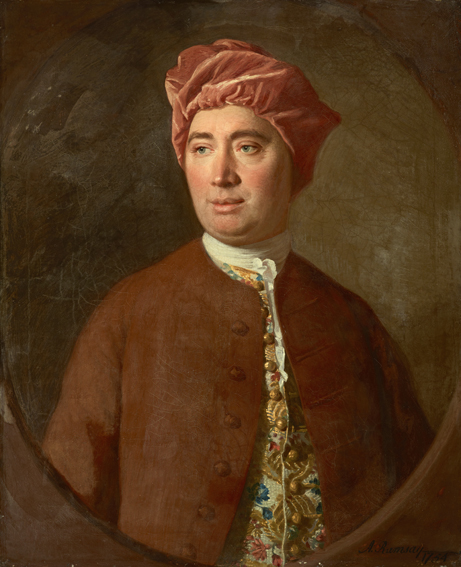
\includegraphics[width=1\linewidth]{./img/hume}
    \end{columns}
\end{frame}

\begin{frame}{Prior Knowledge: How Babys Learn}
    \begin{itemize}
        \item \textbf{Importance of Prosody}\\
            Babys already pay attention to prosody in the womb.
        \item \textbf{Words: They're a Thing}\\
            Babys quickly learn to probabilistically detect word boundaries.
        \item \textbf{Generalizations Between Words}\\
            Once a child realizes that \emph{who} and \emph{which} must be at the beginning of questions, they immediately generalize this to other question words like \emph{when} and \emph{how}.
    \end{itemize}

    \begin{block}{Conclusion}
        Humans are genetically hard-wired to pay attention to specific aspects of language and generalize then in a specific way.
    \end{block}
\end{frame}

\begin{frame}{Prior Knowledge: Lexical Gaps}
    Many concepts are never lexicalized in any languages as they do not represent common human generalization patterns.
    %
    \begin{example}
        \begin{itemize}
            \item taller than half the people in the room
            \item an even number of years old
            \item a word that is its semantic opposite when read backwards
            \item more bulky than heavy
            \item not made in the US
        \end{itemize}
    \end{example}
\end{frame}

\begin{frame}{Prior Knowledge: Non-Existent Generalizations}
    \begin{itemize}
        \item Artificial language learning experiments reveal\\
            how adults reason about language.
        \item Test subject is given new words and examples of their usage.
        \item They must then use the word in new examples.
        \item Words with ``natural'' meanings are learned correctly,\\
            whereas words with unnatural words aren't acquired\\
            even with lots of data.
    \end{itemize}
\end{frame}

\begin{frame}{A Quick Experiment}
    \begin{center}
        \small
        \begin{tabular}{cccccccc}
            
\begin{tikzpicture}
                \fill[blue] (0,0) circle (1em);
            \end{tikzpicture}
            &
            
\begin{tikzpicture}
                \fill[purple] (0,0) circle (1em);
            \end{tikzpicture}
            &
            
\begin{tikzpicture}
                \fill[blue] (0,0) rectangle (2em,2em);
            \end{tikzpicture}
            &
            
\begin{tikzpicture}
                \fill[purple] (0,0) rectangle (2em,2em);
            \end{tikzpicture}
            &
            
\begin{tikzpicture}
                \fill[brown] (0,0) circle (1em);
            \end{tikzpicture}
            &
            
\begin{tikzpicture}
                \fill[brown] (0,0) rectangle (2em,2em);
            \end{tikzpicture}
            &
            
\begin{tikzpicture}
                \fill[brown] (0em,0em) -- (2em,0em) -- (1em,2em) -- cycle;
            \end{tikzpicture}
            \\[6pt]
            \emph{blip}
            &
            not \emph{blip}
            &
            \emph{blip}
            &
            not \emph{blip}
            &
            \visible<2->{%
            \emph{blip}
            }
            &
            \visible<3->{%
            \emph{blip}
            }
            &
            \visible<4->{%
            \emph{blip}
            }
            \\[6pt]
            not \emph{gnok}
            &
            not \emph{gnok}
            &
            \emph{gnok}
            &
            \emph{gnok}
            &
            \visible<6->{%
            \emph{gnok}
            }
            &
            \visible<7->{%
            \emph{gnok}
            }
            &
            \visible<8->{%
            \emph{gnok}
            }
            \\[6pt]
            not \emph{bnik}
            &
            not \emph{bnik}
            &
            \emph{bnik}
            &
            not \emph{bnik}
            &
            \visible<10->{%
            \emph{bnik}
            }
            &
            \visible<11->{%
            \emph{bnik}
            }
            &
            \visible<12->{%
            \emph{bnik}
            }
            \\[6pt]
            \emph{glop}
            &
            \emph{glop}
            &
            not \emph{glop}
            &
            \emph{glop}
            &
            \visible<14->{%
            \emph{glop}
            }
            &
            \visible<15->{%
            \emph{glop}
            }
            &
            \visible<16->{%
            \emph{glop}
            }
            \\[6pt]
            \emph{blok}
            &
            \emph{blok}
            &
            \emph{blok}
            &
            \emph{blok}
            &
            \visible<18->{%
            not \emph{blok}
            }
            &
            \visible<19->{%
            not \emph{blok}
            }
            &
            \visible<20->{%
            not \emph{blok}
            }
        \end{tabular}
    \end{center}

    \begin{description}
        \item[blip] {\visible<5->{not red}}
        \item[gnok] {\visible<9->{brown or rectangular}}
        \item[bnik] {\visible<13->{blip and gnok}}
        \item[glop] {\visible<17->{bnik and if not brown, then not rectangular}}
        \item[blok] {\visible<21->{bnik or glop, but not both}}
    \end{description}
\end{frame}

\begin{frame}{Why Machine Learning is Hard}
    \begin{itemize}
        \item The Gavagai problem is why machine learning is so hard.
        \item No matter how much data you have, it is not enough to tell you the correct way to generalize.
        \item Humans have to tell computers what generalizations\\
            they should entertain.
        \item But for many problems, humans don't know the answer either!
    \end{itemize}
\end{frame}

\begin{frame}{The Machine Learning Recipe}
    All machine learning follows the same procedure:

    \begin{enumerate}
        \item \textbf{Problem}\\
            produce outputs for inputs based on properties $p$, $q$, \ldots\\
            \subpoint{spam filter, face recognition, machine translation}
        \item \textbf{Supervised training}\\
            sample of predefined input-output pairings\\
            \subpoint{spam \& ham emails, photos with names, original \& translated text}
        \item \textbf{Testing}\\
            test performance of model on new test sample
        \item \textbf{Rinse and repeat}\\
            change some parameters of model, train and test again
    \end{enumerate}

    \begin{center}
        \visible<2>{
        But what properties are relevant?\\
        What parameters should be changed?
        }
    \end{center}
\end{frame}

\begin{frame}{The Moral of the Story}
    \begin{itemize}
        \item Any finite amount of input allows for an infinite number of\\
            different generalizations.
        \item But humans mostly generalize in the same ways.
        \item Due to our genetic endowment we are hardwired to generalize\\
            in certain ways but not in others.
        \item A \highlight{computer has no genetic hardwiring},\\
            we must include it in the algorithm.
    \end{itemize}

    \pause
    \begin{alertblock}{Machine Learning in a Nutshell}
        The hard part of machine learning is figuring out the right generalization mechanisms for a given problem.
    \end{alertblock}
\end{frame}


\begin{frame}{Interim Summary}
    \begin{itemize}
        \item Learning always involves prior knowledge\\
            (the generalization strategy).
        \item The reason that we learn what we learn is that we are\\
            genetically hardwired to generalize only in specific ways.
        \item Computers must be given an effective generalization strategy for every new problem.
        \item This is \highlight{hard and takes lots of time}.
    \end{itemize}

    \visible<2>{Whenever things get hard, people start looking for shortcuts\ldots}
\end{frame}

\begin{frame}{A Current Hype: Deep Learning}
    \begin{itemize}
        \item One learning model is all over the media right now:\\
            \highlight{deep learning}
        \item Deep learning = very large and complex neural networks
        \item Neural networks were inspired by the human brain.
    \end{itemize}

    \pause
    \begin{block}{Standard Model of the Human Brain}
        \begin{itemize}
            \item connected network of neurons
            \item input activates neurons, which start ``firing''\\
                (= emitting electrical current)
            \item current activates other neurons $\Rightarrow$ activation patterns
            \item learning = strengthening connection between specific neurons
        \end{itemize}
    \end{block}
\end{frame}

% \begin{frame}{Probabilistic Learning}
%     Real-world learning algorithms are probabilistic.
%     %
%     \begin{block}{The Major Difference}
%         \begin{itemize}
%             \item The Gold paradigm requires perfect learning but allows\\
%                 as much time as needed.
%             \item Probabilistic learning requires fast learning but allows\\
%                 a margin of error.
%         \end{itemize}
%     \end{block}
%
%     \begin{itemize}
%         \item There are \highlight{two kinds of learning error}.
%             \begin{itemize}
%                 \item \textbf{Type 1:} overgeneralizing
%                 \item \textbf{Type 2:} undergeneralizing
%             \end{itemize}
%         \item We can quantify these for probabilistic learners.
%     \end{itemize}
% \end{frame}
%
% \begin{frame}{Precision and Recall}
%     \begin{block}{Reminder: Sound and Complete Learners}
%         \begin{description}
%             \item[sound] algorithm only learns correct things
%             \item[complete] algorithm learns all correct things
%         \end{description}
%     \end{block}
%
%     \pause
%     \begin{block}{Probabilistic Analogues}
%         \begin{description}
%             \item[precision] \% of learned things that are correct
%             \item[recall] \% of correct things that are learned
%         \end{description}
%     \end{block}
%
%     \pause
%     \begin{center}
%         sound = 100\% precision\\
%         complete = 100\% recall
%     \end{center}
% \end{frame}
%
% \begin{frame}{A Real World Example: Medical Tests}
%     Precision and recall often \highlight{do not match our intuitions}.
%
%     \bigskip
%     \textbf{Example:}
%     \begin{itemize}
%         \item Suppose there is a disease that affects about 10\% of the population.
%         \item Your doctor administers a test that has
%             \begin{itemize}
%                 \item 90\% precision,
%                 \item 95\% recall
%             \end{itemize}
%         \item What are the odds that you have the disease if
%             \begin{itemize}
%                 \item your test comes out positive?
%                 \item your test comes out negative?
%             \end{itemize}
%     \end{itemize}
% \end{frame}
%
% \begin{frame}{The Math}
%     \begin{center}
%         \begin{tabular}{r|>{\centering}p{7em}>{\centering}p{7em}|c}
%             & \emph{has disease} & \emph{no disease} & \textbf{total}\\
%             \hline
%             \emph{test positive} & \only<3-6>{true positive} \only<7->{95}& \only<4-8>{false positive}\only<9->{90} & \\
%             \emph{test negative} & \only<5-7>{false negative} \only<8->{5} & \only<6-9>{true negative}\only<10->{810} & \\
%             \hline
%             \textbf{total} & \only<2->{100} & \only<2->{900} & 1000\\
%         \end{tabular}
%     \end{center}
%
%     \bigskip
%     \begin{columns}
%         \column{.5\linewidth}
%         \visible<11->{
%         If test is \textbf{positive}:
%         \begin{align*}
%             \text{P(true positive)} &= \dfrac{95}{1000}\\[9pt]
%             \text{P(positive)} &= \dfrac{95 + 90}{1000}\\[9pt]
%             \text{P(disease)} &= \dfrac{\text{true positive}}{\text{positive}}\\
%                 &\approx 51\%
%         \end{align*}
%         }
%
%         \column{.5\linewidth}
%         \visible<12->{
%         If test is \textbf{negative}:
%         \begin{align*}
%             \text{P(true negative)} &= \dfrac{810}{1000}\\[9pt]
%             \text{P(negative)} &= \dfrac{5 + 810}{1000}\\[9pt]
%             \text{P(disease)} &= 1 - \dfrac{\text{true negative}}{\text{negative}}\\
%                 &\approx 0.6\%
%         \end{align*}
%         }
%     \end{columns}
% \end{frame}
%
% \begin{frame}{Base Rate Neglect}
%     \begin{itemize}
%         \item These probabilities probably surprise you.
%         \item That's because human intuitions are prone to \highlight{base rate neglect}.
%     \end{itemize}
%     %
%     \begin{block}{Base Rate}
%         How frequent is a given event in the whole population\slash sample space?
%     \end{block}
%     %
%     \begin{itemize}
%         \item The low base rate of the disease (10\%) means that even a very accurate test gives many false positives.
%         \item \textbf{Intuition:} Even if you have a really good algorithm, it will not perform all that well if there's many opportunities for it to screw up.
%     \end{itemize}
% \end{frame}
%
% \begin{frame}{The Probabilities with a Base Rate of 50\%}
%     \begin{center}
%         \begin{tabular}{r|>{\centering}p{7em}>{\centering}p{7em}|c}
%             & \emph{has disease} & \emph{no disease} & \textbf{total}\\
%             \hline
%             \emph{test positive} & \only<3-6>{true positive} \only<7->{475}& \only<4-8>{false positive}\only<9->{50} & \\
%             \emph{test negative} & \only<5-7>{false negative} \only<8->{25} & \only<6-9>{true negative}\only<10->{450} & \\
%             \hline
%             \textbf{total} & \only<2->{500} & \only<2->{500} & 1000\\
%         \end{tabular}
%     \end{center}
%
%     \bigskip
%     \begin{columns}
%         \column{.5\linewidth}
%         \visible<11->{
%         If test is \textbf{positive}:
%         \begin{align*}
%             \text{P(true positive)} &= \dfrac{475}{1000}\\[9pt]
%             \text{P(positive)} &= \dfrac{475 + 50}{1000}\\[9pt]
%             \text{P(disease)} &= \dfrac{\text{true positive}}{\text{positive}}\\
%                 &\approx 90\%
%         \end{align*}
%         }
%
%         \column{.5\linewidth}
%         \visible<12->{
%         If test is \textbf{negative}:
%         \begin{align*}
%             \text{P(true negative)} &= \dfrac{450}{1000}\\[9pt]
%             \text{P(negative)} &= \dfrac{25 + 450}{1000}\\[9pt]
%             \text{P(disease)} &= 1 - \dfrac{\text{true negative}}{\text{negative}}\\
%                 &\approx 5\%
%         \end{align*}
%         }
%     \end{columns}
% \end{frame}
%
% \begin{frame}{The Probabilities with a Base Rate of 1\%}
%     \begin{center}
%         \begin{tabular}{r|>{\centering}p{7em}>{\centering}p{7em}|c}
%             & \emph{has disease} & \emph{no disease} & \textbf{total}\\
%             \hline
%             \emph{test positive} & \only<3-6>{true positive} \only<7->{9}& \only<4-8>{false positive}\only<9->{99} & \\
%             \emph{test negative} & \only<5-7>{false negative} \only<8->{1} & \only<6-9>{true negative}\only<10->{891} & \\
%             \hline
%             \textbf{total} & \only<2->{10} & \only<2->{990} & 1000\\
%         \end{tabular}
%     \end{center}
%
%     \bigskip
%     \begin{columns}
%         \column{.5\linewidth}
%         \visible<11->{
%         If test is \textbf{positive}:
%         \begin{align*}
%             \text{P(true positive)} &= \dfrac{9}{1000}\\[9pt]
%             \text{P(positive)} &= \dfrac{9 + 99}{1000}\\[9pt]
%             \text{P(disease)} &= \dfrac{\text{true positive}}{\text{positive}}\\
%                 &\approx 8\%
%         \end{align*}
%         }
%
%         \column{.5\linewidth}
%         \visible<12->{
%         If test is \textbf{negative}:
%         \begin{align*}
%             \text{P(true negative)} &= \dfrac{891}{1000}\\[9pt]
%             \text{P(negative)} &= \dfrac{1 + 891}{1000}\\[9pt]
%             \text{P(disease)} &= 1 - \dfrac{\text{true negative}}{\text{negative}}\\
%                 &\approx 0.1\%
%         \end{align*}
%         }
%     \end{columns}
% \end{frame}
%
% \begin{frame}{The Importance of Base Rate Neglect}
%     \begin{itemize}
%         \item Many medical tests do not offer a statistically significant improvement over the probabilities set by the base rate.
%             Administering them is a waste of money.
%         \item Base rate neglect is often used to pull a fast one on you:
%             \begin{itemize}
%                 \item ``Metal detectors only have an accuracy of 78\%,\\
%                     so we need additional security checks.''
%                 \item ``Standard surveillance techniques for monitoring terrorist communication have a recall of 74\%, so we need deep packet inspection and backdoors in all computers.''
%             \end{itemize}
%     \end{itemize}
% \end{frame}
%
% \begin{frame}{The Psychology of Base Rate Neglect}
%     \begin{itemize}
%         \item Base rate neglect is not a consequence of humans being bad at statistics.
%         \item It all depends on \highlight{how the probabilities are described}.
%     \end{itemize}
%     %
%     \begin{exampleblock}{Rephrasing the Original Probabilities}
%         \begin{itemize}
%             \item 1 out of 10 people have the disease.
%             \item For 1 out of 10 people that do \textbf{not} have the disease,\\
%                 the test will wrongly claim that they do.
%             \item How likely is it that you have the disease if the test is positive?
%         \end{itemize}
%     \end{exampleblock}
% \end{frame}
%
%
% \begin{frame}{Application: Spam Filtering}
%     \begin{description}
%         \item[precision] higher \% $\Rightarrow$ less spam classified as ham
%         \item[recall] higher \%  $\Rightarrow$ less ham classified as spam
%         \item[base rate] how many emails are spam\slash ham?
%     \end{description}
%
%     \begin{block}{Reflecting on Spam Filtering}
%         \begin{itemize}
%             \item What's worse? False positives or false negatives?
%             \item How is this affected by base rate?
%         \end{itemize}
%     \end{block}
% \end{frame}
%
% \begin{frame}{A Spam Classifier: Unigrams With Odds Ratio}
%     probabilistic learner with positive and negative evidence
%     %
%     \begin{description}
%         \item[positive] email is ham
%         \item[negative] email is spam (= not ham)
%     \end{description}
%     %
%     \medskip
%     \textbf{Training the Learner:}
%     \begin{enumerate}
%         \item for each email, calculate unigram counts
%         \item for each unigram \colored{purple}{u}, calculate
%             \begin{itemize}
%                 \item \textbf{\colored{blue}{ham}}(\colored{purple}{u}) = count of \colored{purple}{u} in ham mail
%                 \item \textbf{\colored{orange}{spam}}(\colored{purple}{u}) = count of \colored{purple}{u} in spam mail
%             \end{itemize}
%         \item in addition, calculate
%             \begin{itemize}
%                 \item \textbf{\colored{teal}{ham-words}} = total count of all unigrams in ham mail
%                 \item \textbf{\colored{red}{spam-words}} = total count of words in spam mail
%             \end{itemize}
%         \item for each unigram \colored{purple}{u}, calculate its \textbf{odds ratio}:
%             \[
%                 \dfrac{\textbf{\colored{blue}{ham}(\colored{purple}{u})}}
%                     {\textbf{\colored{teal}{ham-words}}}
%                 :
%                 \dfrac{\textbf{\colored{orange}{spam}(\colored{purple}{u})}}
%                     {\textbf{\colored{red}{spam-words}}}
%             \]
%     \end{enumerate}
% \end{frame}
%
% \begin{frame}{Example: Counts For a Few Emails to Emily}
%     \begin{columns}
%         \column{.4\linewidth}
%         \centering
%         \begin{tabular}{lrr}
%             \toprule
%                & \textbf{\colored{blue}{Ham}} & \textbf{\colored{orange}{Spam}}\\
%             \midrule
%             Emily & 55 & 1\\
%             Hi &   25 & 15\\
%             Dear & 5 & 30\\
%             movie & 3 & 0\\
%             tomorrow & 12 & 2\\
%             Viagra & 0 & 42\\
%             enlargement & 0 & 23\\
%             Nigeria & 0 & 12\\
%             \midrule
%             \textbf{Total} & \colored{teal}{100} & \colored{red}{125}\\
%             \bottomrule
%         \end{tabular}
%
%         \column{.6\linewidth}
%         \begin{itemize}
%             \item Odds ratio for Emily
%             \[
%                 \dfrac{\colored{blue}{55}}{\colored{teal}{100}}
%                 :
%                 \dfrac{\colored{orange}{1}}{\colored{red}{125}}
%                 =
%                 0.55 : 0.008
%                 =
%                 68.75
%             \]
%             \item Odds ratio for Hi
%             \[
%                 \dfrac{\colored{blue}{25}}{\colored{teal}{100}}
%                 :
%                 \dfrac{\colored{orange}{15}}{\colored{red}{125}}
%                 =
%                 0.25 : 0.12
%                 =
%                 2.08
%             \]
%             \item Odds ratio for Dear
%             \[
%                 \dfrac{\colored{blue}{5}}{\colored{teal}{100}}
%                 :
%                 \dfrac{\colored{orange}{30}}{\colored{red}{125}}
%                 =
%                 0.05 : 0.24
%                 =
%                 0.208
%             \]
%         \end{itemize}
%     \end{columns}
% \end{frame}
%
% \begin{frame}{Classifying Spam}
%     \textbf{Classification Algorithm}
%     \begin{enumerate}
%         \item For each email, multiply the odd ratio of its unigram tokens.
%         \item If value is below some threshold, email is spam.
%     \end{enumerate}
%     %
%     \begin{block}{Setting a Threshold}
%         \begin{itemize}
%             \item Default threshold is 1: no bias towards spam\slash ham
%             \item The higher the threshold, the more aggressive the spam filter.\\
%                 \subpoint{mail considered more likely to be spam by default}
%             \item Choice of threshold depends on base rate and user preferences.
%         \end{itemize}
%     \end{block}
% \end{frame}
%
% \begin{frame}{Example: Classifying a Short Email}
%     \textbf{Subject:} Hi\\
%     \textbf{Body:} Hi Dear Emily\\
%
%     \medskip
%     \begin{center}
%         \begin{tabular}{lr}
%             \toprule
%             \textbf{Unigram Tokens} & \textbf{Odd Ratio}\\
%             \midrule
%             Hi & 2.08\\
%             Hi & 2.08\\
%             Dear & 0.208\\
%             Emily & 68.75\\
%             \bottomrule
%         \end{tabular}
%     \end{center}
%
%     \medskip
%     \textbf{Value:}
%         \(
%             2.08 \times 2.08 \times 0.208 \times 68.75 = 61.87
%         \)
%         \\
%     \textbf{Verdict:} \highlight{Ham!}
% \end{frame}

% \begin{frame}{Another Approach: Learning Like the Brain}
%     \begin{itemize}
%         \item Odds ratio learner not too different from what we have seen before\\
%            \subpoint{stylistic analysis, bigram language learner, \ldots}
%         \item Is there something closer to human learning?
%         \item \textbf{Idea:} Take a hint from the \highlight{human brain}!
%     \end{itemize}
%
%     \pause
%     \begin{block}{Standard Model of the Human Brain}
%         \begin{itemize}
%             \item connected network of neurons
%             \item input activates neurons, which start ``firing''\\
%                 (= emitting electrical current)
%             \item current activates other neurons $\Rightarrow$ activation patterns
%             \item learning = strengthening connection between specific neurons
%         \end{itemize}
%     \end{block}
% \end{frame}

\begin{frame}{The Perceptron}
    \begin{block}{The Perceptron: A Mini-Version of a Neural Network}
        \begin{itemize}
            \item \textbf{input layer:} neurons that are sensitive to input
            \item \textbf{output layer:} neurons that represent output values
            \item \textbf{connections:} weighted links between input and output layer
            \item most activated output neuron represents decision
        \end{itemize}
    \end{block}
    %
    \begin{center}
        \begin{tikzpicture}
            \node[minimum size=3em,draw,circle] (dear) at (0,0) {Dear};
            \node[minimum size=3em,draw,circle] (hi) [left=of dear] {Hi};
            \node[minimum size=3em,draw,circle] (emily) [right=of dear] {Emily};
            \node[minimum size=3em,draw,circle] (ham) [below=5em of hi] {ham};
            \node[minimum size=3em,draw,circle] (spam) [below=5em of emily] {spam};

            \foreach \Input/\Output/\Value in {%
                    dear/ham/0,
                    dear/spam/5,
                    hi/ham/3,
                    hi/spam/1,
                    emily/ham/10,
                    emily/spam/0}
                \draw[->] (\Input) to node [right, pos=.75] {\Value} (\Output);
        \end{tikzpicture}
    \end{center}
\end{frame}

\begin{frame}{Perceptron Activation for \emph{Hi Dear}}
    \begin{center}
        \begin{tikzpicture}
            \node[minimum size=3em,draw,circle,fill=blue!25] (dear) at (0,0) {Dear};
            \node[minimum size=3em,draw,circle,fill=blue!25] (hi) [left=of dear] {Hi};
            \node[minimum size=3em,draw,circle] (emily) [right=of dear] {Emily};
            \node[minimum size=3em,draw,circle,fill=red!10] (ham) [below=5em of hi] {ham};
            \node[minimum size=3em,draw,circle,fill=red!35] (spam) [below=5em of emily] {spam};

            \foreach \Input/\Output/\Value in {%
                    dear/ham/0,
                    dear/spam/5,
                    hi/ham/3,
                    hi/spam/1,
                    emily/ham/10,
                    emily/spam/0}
                \draw[->] (\Input) to node [right, pos=.75] {\Value} (\Output);
        \end{tikzpicture}
    \end{center}
\end{frame}

\begin{frame}{Perceptron Activation for \emph{Hi Dear Emily}}
    \begin{center}
        \begin{tikzpicture}
            \node[minimum size=3em,draw,circle,fill=blue!25] (dear) at (0,0) {Dear};
            \node[minimum size=3em,draw,circle,fill=blue!25] (hi) [left=of dear] {Hi};
            \node[minimum size=3em,draw,circle,fill=blue!25] (emily) [right=of dear] {Emily};
            \node[minimum size=3em,draw,circle,fill=red!75] (ham) [below=5em of hi] {ham};
            \node[minimum size=3em,draw,circle,fill=red!35] (spam) [below=5em of emily] {spam};

            \foreach \Input/\Output/\Value in {%
                    dear/ham/0,
                    dear/spam/5,
                    hi/ham/3,
                    hi/spam/1,
                    emily/ham/10,
                    emily/spam/0}
                \draw[->] (\Input) to node [right, pos=.75] {\Value} (\Output);
        \end{tikzpicture}
    \end{center}
\end{frame}

\begin{frame}{Training the Perceptron}
    The perceptron learns in a strange way:

    \medskip
    \begin{enumerate}
        \item \textbf{Rewiring Step}\\
                if output is wrong, randomly change weights of links
        \item \textbf{Evaluation Step}
            \begin{itemize}
                \item if output is closer to intended result, keep new weights
                \item otherwise keep previous weights
            \end{itemize}
        \item \textbf{Iteration Step}\\
                if output is still wrong, return to first step
    \end{enumerate}

    \medskip
    \begin{center}
        \visible<2>{
            \highlight{Learning = Iterated Trial and Error}
        }
    \end{center}
\end{frame}

\begin{frame}{What Can be Learned: Linear Separability}
    \begin{theorem}[Perceptron Learning]
        A target class can be learned perfectly by the perceptron\\
        if and only if
        it is \textbf{linearly separable}.
    \end{theorem}
    %
    \begin{description}
        \item[linearly separable] target class can be delineated by a single line
    \end{description}
    %
    \begin{center}
        \begin{tikzpicture}[
            good/.style = {draw=blue!50, fill=blue!50, inner sep=0pt, minimum size=.2em, circle},
            bad/.style = {draw=red!50, fill=red!50, inner sep=0pt, minimum size=.2em, circle}
            ]
            \draw[->] (0,0) to (12em,0);
            \draw[->] (0,0) to (0,10em);

            \draw[thick,purple,visible on=<2>,xshift=.2em,yshift=.2em] (12em,-2em) to (-3em,10em);

            \foreach \X/\Y in {%
                7/5,
                10/7.3,
                11/1,
                1/9,
                .25/8,
                6/2}
                \node[good] at (\X em, \Y em) {};

            \foreach \X/\Y in {%
                1/1,
                3/.5,
                8/.2,
                1.6/6.5,
                6.1/2.5}
                \node[bad] at (\X em, \Y em) {};
        \end{tikzpicture}
    \end{center}
\end{frame}

\begin{frame}{Example: Calculating Truth}
    \begin{tabular}{ccc}
        \begin{tikzpicture}[
                good/.style = {draw=blue!50, fill=blue!50, inner sep=0pt, minimum size=.5em, circle},
                bad/.style = {draw=red!50, fill=red!50, inner sep=0pt, minimum size=.5em, circle}
                ]
                \node (F) at (0,0) {F};
                \node (Tx) [right=6em of F] {T};
                \node (Ty) [above=6em of F] {T};
                \draw (F.north east) to (Tx.north);
                \draw (F.north east) to (Ty.east);

                % dots
                \node[bad] at (F.north east) {};
                \node[bad] at (Ty.east) {};
                \node[bad] at (Tx.north) {};
                \node[good] at (Ty.east -| Tx.north) {};

                % label
                \node at ($(F.south) !.5! (Tx.south)$) [font=\bfseries]
                    {and};

                % separator
                \draw[thick,purple,visible on=<2->] (8.5em,0em) to (0em,8.5em);
        \end{tikzpicture}
        &
        \begin{tikzpicture}[
                good/.style = {draw=blue!50, fill=blue!50, inner sep=0pt, minimum size=.5em, circle},
                bad/.style = {draw=red!50, fill=red!50, inner sep=0pt, minimum size=.5em, circle}
                ]
                \node (F) at (0,0) {F};
                \node (Tx) [right=6em of F] {T};
                \node (Ty) [above=6em of F] {T};
                \draw (F.north east) to (Tx.north);
                \draw (F.north east) to (Ty.east);

                % dots
                \node[bad] at (F.north east) {};
                \node[good] at (Ty.east) {};
                \node[good] at (Tx.north) {};
                \node[good] at (Ty.east -| Tx.north) {};

                % label
                \node at ($(F.south) !.5! (Tx.south)$) [font=\bfseries]
                    {or};

                % separator
                \draw[thick,purple,visible on=<3->] (7em,-1em) to (-1em,7em);
        \end{tikzpicture}
        &
        \begin{tikzpicture}[
                good/.style = {draw=blue!50, fill=blue!50, inner sep=0pt, minimum size=.5em, circle},
                bad/.style = {draw=red!50, fill=red!50, inner sep=0pt, minimum size=.5em, circle}
                ]
                \node (F) at (0,0) {F};
                \node (Tx) [right=6em of F] {T};
                \node (Ty) [above=6em of F] {T};
                \draw (F.north east) to (Tx.north);
                \draw (F.north east) to (Ty.east);

                % dots
                \node[bad] at (F.north east) {};
                \node[good] at (Ty.east) {};
                \node[good] at (Tx.north) {};
                \node[bad] at (Ty.east -| Tx.north) {};

                % label
                \node at ($(F.south) !.5! (Tx.south)$) [font=\bfseries]
                    {xor};
        \end{tikzpicture}
    \end{tabular}
\end{frame}

\begin{frame}{Improving the Perceptron: Neural Network}
    Perceptron is too weak for classes that are not linearly separable.
    
    \begin{block}{Neural Networks and Deep Learning}
        Neural networks extend the perceptron with
        %
        \begin{itemize}
            \item intermediate layers, and
            \item feedback loops between layers.
        \end{itemize}
        %
        \textbf{Deep learning} uses neural networks with dozens of layers\\
        $\Rightarrow$ no revolutionary techniques, just super-sizing old ideas
    \end{block}
\end{frame}

\begin{frame}{Why Neural Networks are Loved and Hated}
    Neural networks are a \highlight{tremendous improvement} because
    \begin{itemize}
        \item they work surprsingly well with no explicit guidance;
        \item they work across many different domains;\\
            \subpoint{machine translation, melanoma diagnosis, self-driving car}
        \item instead of understanding the problem,\\
            we can brute-force it with trial and error.
    \end{itemize}
    Neural networks are \highlight{unsatisfying} because
    \begin{itemize}
        \item they are too complex to tell what is going on;
        \item it is all trial-and-error with shaky theoretical foundation;
        \item there are no safeties or learning guarantees;
        \item minor changes in data or model can have huge effects.
    \end{itemize}
\end{frame}

\begin{frame}{Is the Brain a Perceptron\slash Neural Network?}
    \begin{alertblock}{A Nasty Truth}
        We have no idea how the brain computes!
    \end{alertblock}

    \begin{itemize}
        \item The physiology of the brain has limited bearing on computation:
            %
            \begin{itemize}
                \item a program can have very different hardware instantiations
                \item a hardware activation can compute very different things
            \end{itemize}
        \item The physiology of the brain is open to interpretation:
            \begin{itemize}
                \item Do neurons have activation levels?
                \item Computer transistors only have two states (on and off)\\
                    despite the range of transistor voltages being almost infinite.
            \end{itemize}
    \end{itemize}

    \pause
    \begin{block}{The Real-World Failure}
        \begin{itemize}
            \item We have a full ``brain map'' of roundworm \emph{C. elegans}.
            \item 302 neurons and links between them
            \item Yet we have no idea how this brain works!
        \end{itemize}
    \end{block}
\end{frame}

\begin{frame}{A Different View of Neural Computation}
    \begin{columns}
        \column{.7\linewidth}
        \textbf{Randy Gallistel} (Psychologist@Rutgers)
        \begin{itemize}
            \item Neuroscience has it all wrong.
            \item We need theory of computation.
            \item Good starting point:\\
                Memory data structures?\\
                How are they instantiated?
        \end{itemize}

        \bigskip
        Check out the \textbf{Brain Science Podcast}\\
        \smallskip
        \url{https://www.youtube.com/playlist?list=PLUSRfoOcUe4bf0ly1WSvxagPiG3569Al1}

        \column{.3\linewidth}
        \centering
        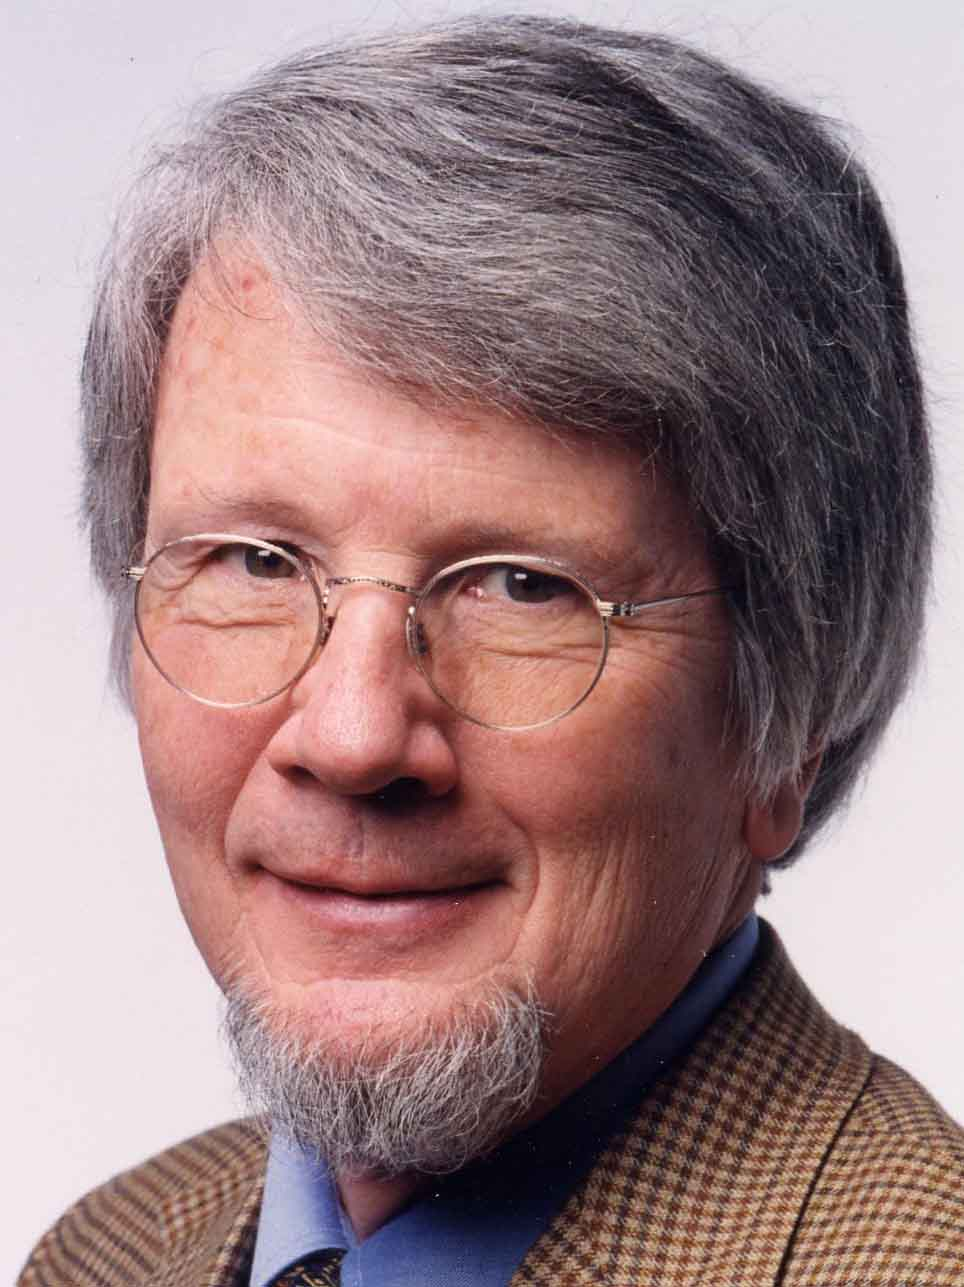
\includegraphics[width=6em]{./img/gallistel}\\
        \medskip
        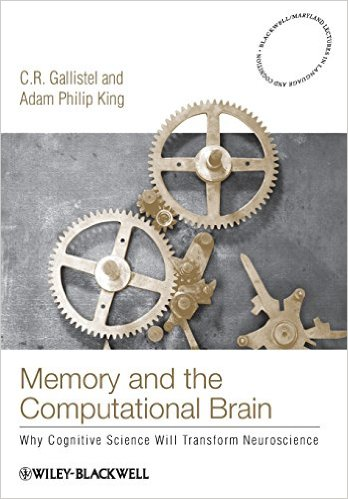
\includegraphics[width=6em]{./img/gallistelkingbook}
    \end{columns}
\end{frame}

\begin{frame}{Zipf's Law Strikes Again!}
    \begin{itemize}
        \item Neural networks have a bigger problem than cognitive reality:\\
            \highlight{Zipf's Law!}
        \item Many constructions in language are excessively rare.
        \item Neural networks rely on iterated trial and error\\
            $\Rightarrow$ stabilization is driven by common inputs
        \item When push comes to shove, a neural network will\\
            maximize performance over common inputs\\
            at the expense of rare inputs.
    \end{itemize}

    \pause
    \begin{block}{Moral of the Story}
        \begin{itemize}
            \item Deep learning is all the rage now.
            \item But it is unlikely that it will solve the problem of\\
                language learning. 
        \end{itemize}
    \end{block}
\end{frame}

\end{document}
